\documentclass[11pt]{article}
%Gummi|065|=)
\usepackage{graphicx,url}
\usepackage[utf8]{inputenc}
\usepackage[brazil]{babel}
\usepackage{graphicx}
\title{\textbf{Trabalho Prático II - Indexador}}
\author{Thiago Vieira de Alcantara Silva\\2012075627}
\date{}
\begin{document}

\maketitle

\section{Introdução}
Neste trabalho, desenvolvi um indexador e um processador de consultas simples. Dado um conjunto de páginas web, o indexador as analisa, retira todos os termos presentes em seus conteúdos e cria um arquivo invertido, onde cada linha representa um termo e contém pares indicando em qual documento podemos encontrar o termo e quantas vezes ele aparece no documento. O processador de consultas foi desenvolvido seguindo o modelo booleano, assim as consultas são realizadas somente verificando se os termos da consulta estão presentes nos documentos; o ranking dos documentos é dado pelo número que termos da consulta que eles contém.

\section{Decisões de Projeto}
\subsection{Estrutura do Projeto}
Tanto o indexador como o processador de consultas foram desenvolvidos em C++.
A pasta principal do projeto é dividida em oito pastas diferentes:
\begin{itemize}
\item bin: Pasta onde os binários do indexador se localizam.
\item doc: Pasta para guardar a descrição e documentação do projeto.
\item documents: Pasta que uso para guardar sets de páginas web, uso não obrigatório.
\item gumbo-parser: Pasta presente no indexador, onde a biblioteca gumbo é armazenada.
\item output: Pasta onde os arquivos finais se localizam, dentre eles estão o index, urls e vocabulary$\_$l, onde guardo, respectivamente, o arquivo invertido, a lista de urls e o vocabulário ordenado lexicograficamente.
\item src: Pasta onde guardo o código fonte do indexador.
\item tst: Pasta onde ficam os testes realizados para aprender as interfaces das bibliotecas usadas e para avaliar a corretude e eficiência de partes do código.
\item .tmp: Pasta usada para guardar arquivos temporários necessários para o indexador.
\end{itemize}


\subsection{Bibliotecas, Dependências e Execução}
Os pacotes necessários para executar o indexador são gumbo-parser e libicu. O gumbo-parser  é uma biblioteca desenvolvida pela Google ( \url{http://github.com/google/gumbo-parser} ), usada para fazer o parsing das páginas web e a libicu é utilizada para retirar caracteres especiais dos documentos.\\
Um shell script, install.sh, foi desenvolvido para checar se o sistema operacional contém os pacotes e os instala se necessário.
Para facilitar a compilação do indexador foi criado um snippet usando o utilitário Makefile, logo para compilar o código basta executar um make que o objeto main aparecerá na pasta principal.\\
No arquivo DOCFILENAMES está localizada a lista dos nomes dos arquivos onde estão as páginas web, não é necessário passar este arquivo para o executável do indexador. Ao iniciar, o indexador lê os nomes dos arquivos de DOCFILENAMES, os armazena e começa o processo de indexação.


\subsection{Método de Ordenação Externa}
Após a geração das triplas, um algoritmo de ordenação entra em ação. Para ordenar o arquivos das triplas foi usado o heap-sort multiway, assim ordenamos chunks do arquivo de triplas e os salvamos em arquivos separados, logo após, uma intercalação desses arquivos é executada gerando o arquivo final ordenado.


\subsection{Paralelismo}
A geração de triplas de cada documento é feita em duas partes, o parsing do documento e a escrita das triplas em disco, uma vez em que o parsing do documento foi executado podemos escrever as triplas no arquivo de saída, assim podemos executar a geração das triplas usando duas threads, simulando um pipeline. O gargalo deste processo se encontra nas escritas em disco, assim o pipeline se comporta como mostrado na imagem abaixo:


%\begin{figure}
%\centering
%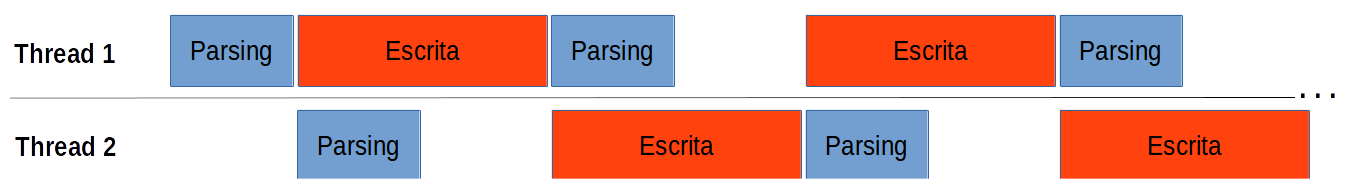
\includegraphics[width=0.8\textwidth,scale=0.41,natwidth=1354,natheight=192]{Pipelining.png}
%\end{figure}

Assim, aproveitamos o máximo do tempo, sempre fazendo parsing e escrevendo em disco.


\section{Análise de Complexidade}

\subsection{Memória}

Os módulos que gastam mais memória são vocabulário e externalsorter. O módulo responsável pelo vocabulário armazena o equivalente a duas vezes o número de termos da base de páginas, isso equivale em média a 10$\%$ do tamanho total das páginas.\\
Externalsorter tem um limite de memória interna para ser usado, o limite pode ser alterado chamando o método SetMemoryLimit. O padrão é 128Mb, coloquei este limite considerando a quantidade de memória que os buffers de fstream gastam, além do fato dos containers da stl dobrarem de tamanho a cada vez que seus limites são atingidos.

\subsection{Tempo}
Os atos que requerem maior tempo de execução são a geração das triplas e a ordenação delas.\\
A geração das triplas é feita executando um parsing dos documentos, usando a biblioteca gumbo, e escrevendo as triplas em um arquivo. Assumindo que gumbo executa o parsing em tempo linear, a geração das triplas é executada em O($n$ $log n$) onde $n$ é o número de termos; existe um fator log n pois contamos a frequência de cada termo nos documentos.\\
A ordenação das triplas é feita usando o multiway heap-sort. Sendo $T$ o total de triplas geradas e $m$ o máximo de triplas armazenadas em memória principal, temos a complexidade total da ordenação O(T log T), o número de chunks criados na ordenação $\lceil T/m \rceil$.


\section{Resultados Experimentais}
Os testes foram executados em um Intel® Core i5-4210U CPU @ 1.70GHz x 4.

\subsection{Ordenação Externa}
Foram executados testes para verificar a eficiência do método de ordenação externa usado neste trabalho. Os testes foram executados com arquivos de 100 a 10.000.000 triplas, e usando desde 100Kb de memória interna até 128Mb.

%
%\begin{figure}
%\centering
%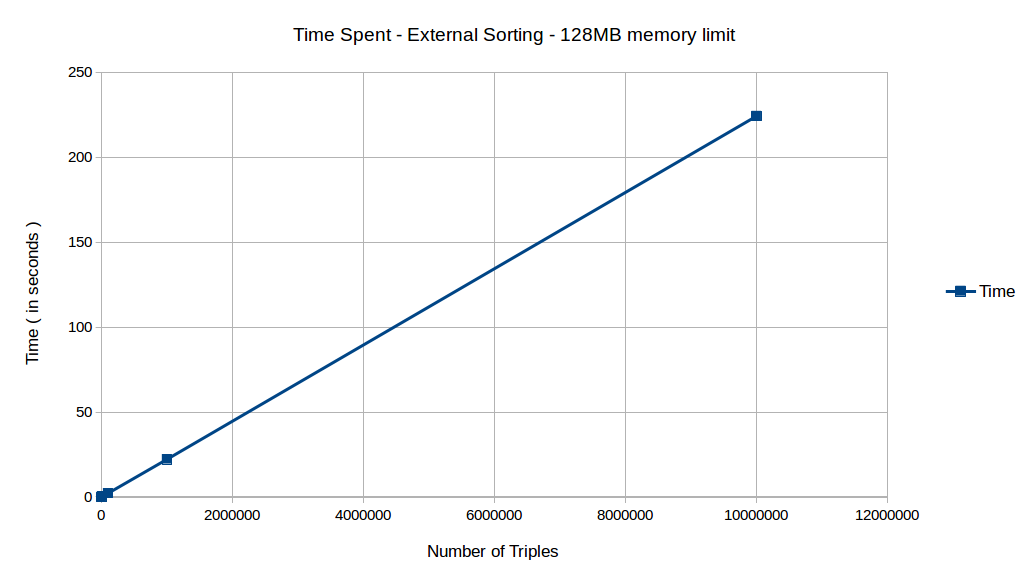
\includegraphics[width=0.7\textwidth,scale=0.5,natwidth=1024,natheight=581]{ExternalSortingEfficiency.png}
%\end{figure}

Apesar da variação da memória interna máxima nos testes, o resultado foi idêntico para todos; isso talvez se dê pelo fato de sempre termos o stream de todos os chunks abertos na ordenação.

\subsection{Indexação}

Foram executados testes para verificar a eficiência do indexador como um todo. Os testes foram executados com 4 bases, com 141, 601, 2078 e 10096 documentos.

%\begin{figure}
%\centering
%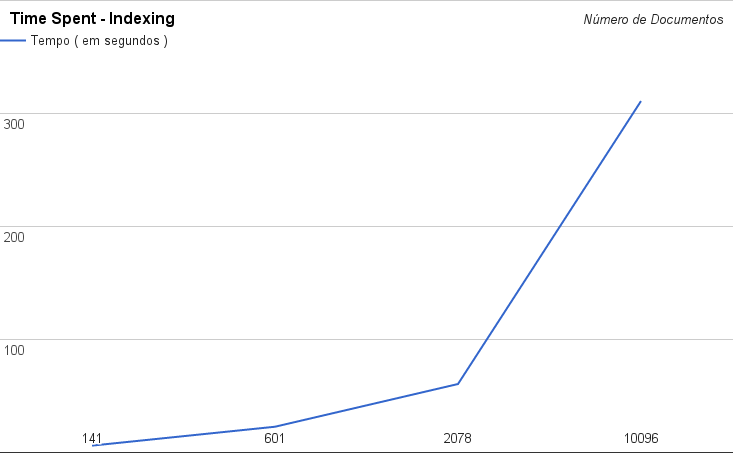
\includegraphics[width=0.7\textwidth,scale=0.5,natwidth=1029,natheight=192]{IndexingEfficiency.png}
%\end{figure}

Com esses dois testes apresentados, é possível verificar que o indexador passa o maior tempo tratando os documentos e escrevendo as triplas do que ordenando-as. Assim uma possível otimização do indexador deveria focar na primeira fase da indexação.


\end{document}
